\documentclass{standalone}
\usepackage{tikz}
\usetikzlibrary{patterns, positioning}


\begin{document}
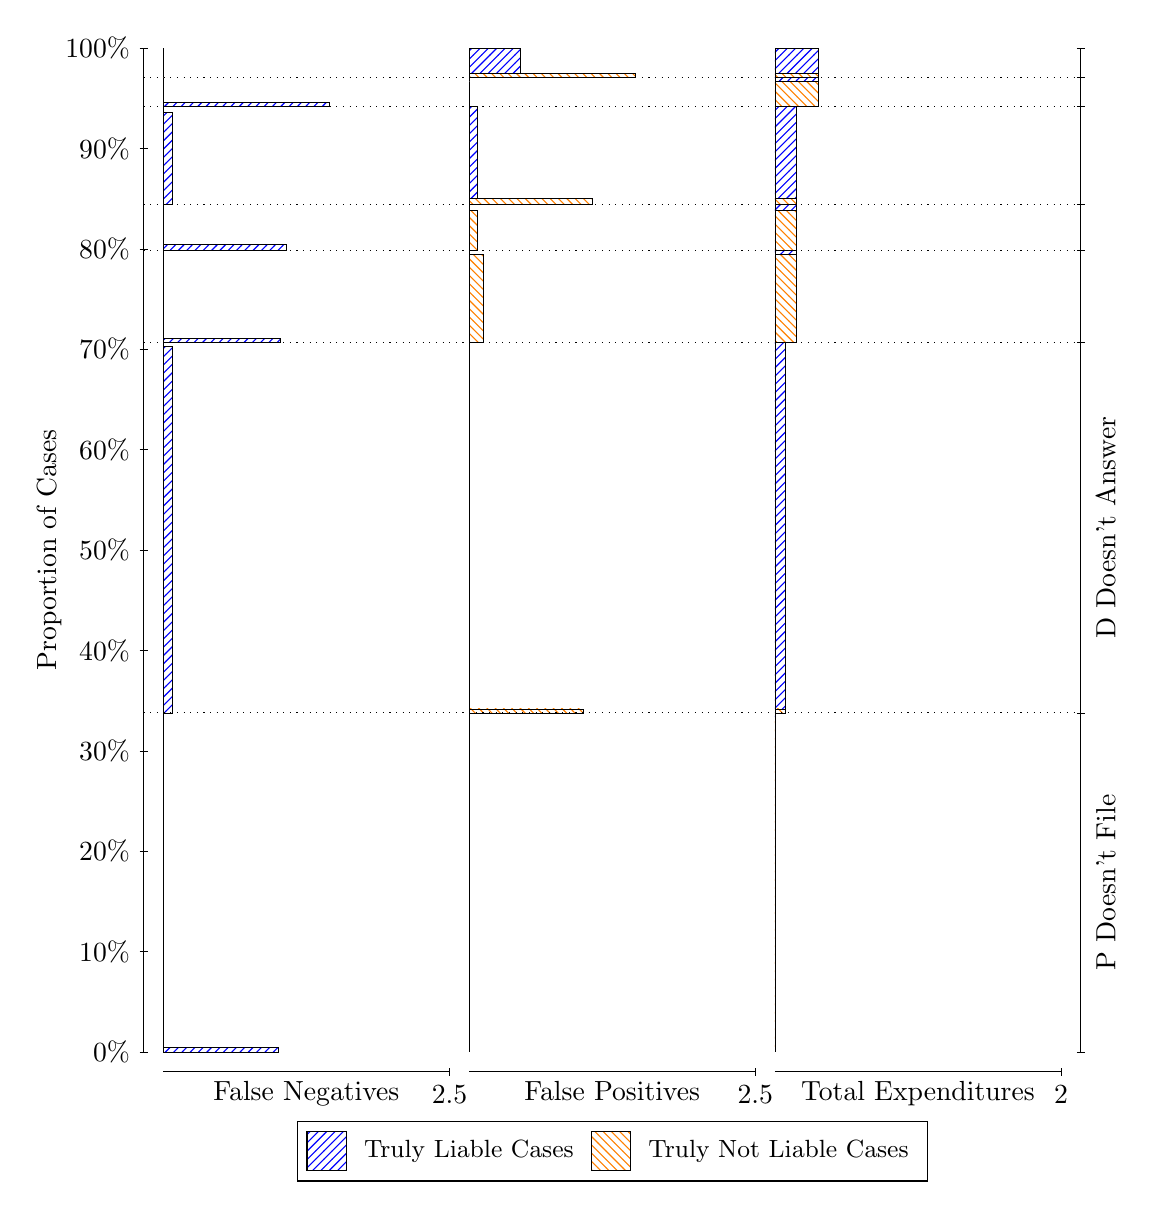
\begin{tikzpicture}
\draw[black, very thin] (1.5,1.75) -- (1.5,14.5);
\node[rotate=90, text=black, anchor=center] at (0.3, 8.125) {Proportion of Cases};
\draw[black, very thin] (1.45,1.75) -- (1.55,1.75);
\node[text=black, anchor=east] at (1.45, 1.75) {0\%};
\draw[black, very thin] (1.45,3.025) -- (1.55,3.025);
\node[text=black, anchor=east] at (1.45, 3.025) {10\%};
\draw[black, very thin] (1.45,4.3) -- (1.55,4.3);
\node[text=black, anchor=east] at (1.45, 4.3) {20\%};
\draw[black, very thin] (1.45,5.575) -- (1.55,5.575);
\node[text=black, anchor=east] at (1.45, 5.575) {30\%};
\draw[black, very thin] (1.45,6.85) -- (1.55,6.85);
\node[text=black, anchor=east] at (1.45, 6.85) {40\%};
\draw[black, very thin] (1.45,8.125) -- (1.55,8.125);
\node[text=black, anchor=east] at (1.45, 8.125) {50\%};
\draw[black, very thin] (1.45,9.4) -- (1.55,9.4);
\node[text=black, anchor=east] at (1.45, 9.4) {60\%};
\draw[black, very thin] (1.45,10.675) -- (1.55,10.675);
\node[text=black, anchor=east] at (1.45, 10.675) {70\%};
\draw[black, very thin] (1.45,11.95) -- (1.55,11.95);
\node[text=black, anchor=east] at (1.45, 11.95) {80\%};
\draw[black, very thin] (1.45,13.225) -- (1.55,13.225);
\node[text=black, anchor=east] at (1.45, 13.225) {90\%};
\draw[black, very thin] (1.45,14.5) -- (1.55,14.5);
\node[text=black, anchor=east] at (1.45, 14.5) {100\%};

\draw[black, very thin] (13.4,1.75) -- (13.4,14.5);
\draw[black, very thin] (13.35,1.75) -- (13.45,1.75);
\node[anchor=west] at (13.35, 1.75) {};
\draw[black, very thin] (13.35,6.0565) -- (13.45,6.0565);
\node[anchor=west] at (13.35, 6.0565) {};
\draw[black, very thin] (13.35,10.761) -- (13.45,10.761);
\node[anchor=west] at (13.35, 10.761) {};
\draw[black, very thin] (13.35,11.932) -- (13.45,11.932);
\node[anchor=west] at (13.35, 11.932) {};
\draw[black, very thin] (13.35,12.512) -- (13.45,12.512);
\node[anchor=west] at (13.35, 12.512) {};
\draw[black, very thin] (13.35,13.756) -- (13.45,13.756);
\node[anchor=west] at (13.35, 13.756) {};
\draw[black, very thin] (13.35,14.128) -- (13.45,14.128);
\node[anchor=west] at (13.35, 14.128) {};
\draw[black, very thin] (13.35,14.5) -- (13.45,14.5);
\node[anchor=west] at (13.35, 14.5) {};

\draw[black, very thin, pattern color=blue, pattern=north east lines] (1.75,1.75) rectangle (3.2033,1.8037);
\draw[black, very thin, pattern color=orange, pattern=north west lines] (1.75,1.8037) rectangle (1.75,6.0565);
\draw[black, very thin, pattern color=blue, pattern=north east lines] (1.75,6.0565) rectangle (1.859,10.71);
\draw[black, very thin, pattern color=orange, pattern=north west lines] (1.75,10.71) rectangle (1.75,10.761);
\draw[black, very thin, pattern color=blue, pattern=north east lines] (1.75,10.761) rectangle (3.2397,10.817);
\draw[black, very thin, pattern color=orange, pattern=north west lines] (1.75,10.817) rectangle (1.75,11.932);
\draw[black, very thin, pattern color=blue, pattern=north east lines] (1.75,11.932) rectangle (3.3123,12.003);
\draw[black, very thin, pattern color=orange, pattern=north west lines] (1.75,12.003) rectangle (1.75,12.512);
\draw[black, very thin, pattern color=blue, pattern=north east lines] (1.75,12.512) rectangle (1.859,13.681);
\draw[black, very thin, pattern color=orange, pattern=north west lines] (1.75,13.681) rectangle (1.75,13.756);
\draw[black, very thin, pattern color=blue, pattern=north east lines] (1.75,13.756) rectangle (3.8573,13.808);
\draw[black, very thin, pattern color=orange, pattern=north west lines] (1.75,13.808) rectangle (1.75,14.128);
\draw[black, very thin, pattern color=orange, pattern=north west lines] (1.75,14.128) rectangle (1.75,14.18);
\draw[black, very thin, pattern color=blue, pattern=north east lines] (1.75,14.18) rectangle (1.75,14.5);
\draw[black, very thin, pattern color=orange, pattern=north west lines] (5.6333,1.75) rectangle (5.6333,6.0028);
\draw[black, very thin, pattern color=blue, pattern=north east lines] (5.6333,6.0028) rectangle (5.6333,6.0565);
\draw[black, very thin, pattern color=orange, pattern=north west lines] (5.6333,6.0565) rectangle (7.0867,6.1076);
\draw[black, very thin, pattern color=blue, pattern=north east lines] (5.6333,6.1076) rectangle (5.6333,10.761);
\draw[black, very thin, pattern color=orange, pattern=north west lines] (5.6333,10.761) rectangle (5.815,11.876);
\draw[black, very thin, pattern color=blue, pattern=north east lines] (5.6333,11.876) rectangle (5.6333,11.932);
\draw[black, very thin, pattern color=orange, pattern=north west lines] (5.6333,11.932) rectangle (5.7423,12.44);
\draw[black, very thin, pattern color=blue, pattern=north east lines] (5.6333,12.44) rectangle (5.6333,12.512);
\draw[black, very thin, pattern color=orange, pattern=north west lines] (5.6333,12.512) rectangle (7.1957,12.587);
\draw[black, very thin, pattern color=blue, pattern=north east lines] (5.6333,12.587) rectangle (5.7423,13.756);
\draw[black, very thin, pattern color=orange, pattern=north west lines] (5.6333,13.756) rectangle (5.6333,14.076);
\draw[black, very thin, pattern color=blue, pattern=north east lines] (5.6333,14.076) rectangle (5.6333,14.128);
\draw[black, very thin, pattern color=orange, pattern=north west lines] (5.6333,14.128) rectangle (7.7407,14.18);
\draw[black, very thin, pattern color=blue, pattern=north east lines] (5.6333,14.18) rectangle (6.2873,14.5);
\draw[black, very thin, pattern color=orange, pattern=north west lines] (9.5167,1.75) rectangle (9.5167,6.0028);
\draw[black, very thin, pattern color=blue, pattern=north east lines] (9.5167,6.0028) rectangle (9.5167,6.0565);
\draw[black, very thin, pattern color=orange, pattern=north west lines] (9.5167,6.0565) rectangle (9.6529,6.1076);
\draw[black, very thin, pattern color=blue, pattern=north east lines] (9.5167,6.1076) rectangle (9.6529,10.761);
\draw[black, very thin, pattern color=orange, pattern=north west lines] (9.5167,10.761) rectangle (9.7892,11.876);
\draw[black, very thin, pattern color=blue, pattern=north east lines] (9.5167,11.876) rectangle (9.7892,11.932);
\draw[black, very thin, pattern color=orange, pattern=north west lines] (9.5167,11.932) rectangle (9.7892,12.44);
\draw[black, very thin, pattern color=blue, pattern=north east lines] (9.5167,12.44) rectangle (9.7892,12.512);
\draw[black, very thin, pattern color=orange, pattern=north west lines] (9.5167,12.512) rectangle (9.7892,12.587);
\draw[black, very thin, pattern color=blue, pattern=north east lines] (9.5167,12.587) rectangle (9.7892,13.756);
\draw[black, very thin, pattern color=orange, pattern=north west lines] (9.5167,13.756) rectangle (10.062,14.076);
\draw[black, very thin, pattern color=blue, pattern=north east lines] (9.5167,14.076) rectangle (10.062,14.128);
\draw[black, very thin, pattern color=orange, pattern=north west lines] (9.5167,14.128) rectangle (10.062,14.18);
\draw[black, very thin, pattern color=blue, pattern=north east lines] (9.5167,14.18) rectangle (10.062,14.5);
\draw[black, dotted] (1.5,6.0565) -- (13.4,6.0565);
\draw[black, dotted] (1.5,10.761) -- (13.4,10.761);
\draw[black, dotted] (1.5,11.932) -- (13.4,11.932);
\draw[black, dotted] (1.5,12.512) -- (13.4,12.512);
\draw[black, dotted] (1.5,13.756) -- (13.4,13.756);
\draw[black, dotted] (1.5,14.128) -- (13.4,14.128);
\draw[black, very thin] (1.75,1.5) -- (5.3833,1.5);
\node[text=black, anchor=north] at (3.5667, 1.5) {False Negatives};
\draw[black, very thin] (5.3833,1.45) -- (5.3833,1.55);
\node[text=black, anchor=north] at (5.3833, 1.45) {2.5};

\draw[black, very thin] (5.6333,1.5) -- (9.2667,1.5);
\node[text=black, anchor=north] at (7.45, 1.5) {False Positives};
\draw[black, very thin] (9.2667,1.45) -- (9.2667,1.55);
\node[text=black, anchor=north] at (9.2667, 1.45) {2.5};

\draw[black, very thin] (9.5167,1.5) -- (13.15,1.5);
\node[text=black, anchor=north] at (11.333, 1.5) {Total Expenditures};
\draw[black, very thin] (13.15,1.45) -- (13.15,1.55);
\node[text=black, anchor=north] at (13.15, 1.45) {2};

\node[text=black, centered, rotate=90] at (13.72, 3.9033) {P Doesn't File};
\node[text=black, centered, rotate=90] at (13.72, 8.409) {D Doesn't Answer};






\draw (7.449999999999999,1.5) node[draw=none] (baseCoordinate) {};
\begin{scope}[align=center]
        \matrix[scale=0.5, draw=black, below=0.5cm of baseCoordinate, nodes={draw}, column sep=0.1cm]{
            \node[rectangle, draw, minimum width=0.5cm, minimum height=0.5cm, pattern color=blue, pattern=north east lines] {}; &
            \node[draw=none, font=\small, text=black] (B) {Truly Liable Cases}; &
            \node[rectangle, draw, minimum width=0.5cm, minimum height=0.5cm, pattern color=orange, pattern=north west lines] {}; &
            \node[draw=none, font=\small, text=black] (B) {Truly Not Liable Cases}; \\
            };
\end{scope}

\end{tikzpicture}
\end{document}